% standalone wrapper for a tikz picture
\documentclass[tikz,border=2pt]{standalone}
\usepackage{xcolor}
\usepackage{tikz}
\usetikzlibrary{shapes,arrows,positioning,shadows,patterns,arrows.meta,calc}
\definecolor{cwAlert}{RGB}{220,50,50}
\definecolor{cwFlow}{RGB}{50,120,220}
\definecolor{cwDecoy}{RGB}{120,180,50}
\definecolor{cwBorder}{RGB}{80,80,80}
\definecolor{ImperialBlue}{RGB}{0,62,116}
\definecolor{ImperialNavy}{RGB}{0,33,71}
\definecolor{ImperialLightBlue}{RGB}{155,203,235}
\begin{document}

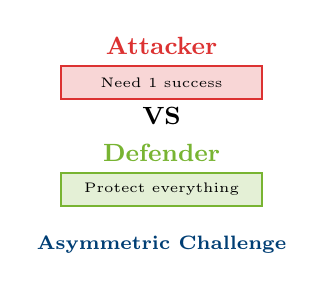
\begin{tikzpicture}[scale=0.85]
    % Attacker side (top)
    \node[font=\small\bfseries] at (1.5,2.3) {\textcolor{cwAlert}{Attacker}};
    \draw[fill=cwAlert!20, draw=cwAlert, thick] (0,2) rectangle (3,1.5);
    \node[align=center, font=\tiny] at (1.5,1.75) {Need 1 success};
    
    % VS in middle
    \node[font=\small\bfseries] at (1.5,1.25) {VS};
    
    % Defender side (bottom)
    \node[font=\small\bfseries] at (1.5,0.7) {\textcolor{cwDecoy}{Defender}};
    \draw[fill=cwDecoy!20, draw=cwDecoy, thick] (0,0.4) rectangle (3,-0.1);
    \node[align=center, font=\tiny] at (1.5,0.15) {Protect everything};
    
    % Asymmetric indicator
    \node[below, font=\scriptsize\bfseries] at (1.5,-0.4) {\textcolor{ImperialBlue}{Asymmetric Challenge}};
\end{tikzpicture}
\end{document}
